%%%%%%%%%%%%%%%%%%%%%%%%%%%%%%%%%%%%%%%%%%%%%%%%%%%%%%%%%%%%%%%%%%%%%%%%%%%%%%%%%
% Implementación
%%%%%%%%%%%%%%%%%%%%%%%%%%%%%%%%%%%%%%%%%%%%%%%%%%%%%%%%%%%%%%%%%%%%%%%%%%%%%%%%%

\chapter{Implementación de la propuesta}
\label{cha:Implementacion}

    \section{Reproducción de sonido} % (fold)
    \label{sec:ReproduccionDeSonido}

        La reproducción del sonido se realiza utilizando las dos bibliotecas mencionadas en el capítulo
        anterior \ref{sub:LibreriaDeReproduccionDeSonido}, mpg123 y libao.

        El proceso completo que se sigue desde que se pulsa uno de los sensores hasta que se reproduce el sonido es el
        siguiente:
        \begin{enumerate}
            \item Uno de los sensores de presión realiza una lectura y manda el valor leído a la placa Arduino.
            \item El Arduino, prepara un mensaje que escribe en el log del monitor serie (\ref{sec:SonidoEnParalelo}).
            \item La función \texttt{readSerial} lee de \textit{/dev/ttyACM0}, la salida del monitor serie, filtra que
            no sea un mensaje vacío o de que no hay que reproducir nada y se manda a parsear.
            \item En \texttt{parseInstruments} se procesa el mensaje leído.
            \item En la función \texttt{PressToPlay} se selecciona qué instrumento debe sonar.
            \item Finalmente, en la función \texttt{play}, se descodifica el archivo de sonido correspondiente y se
            reproduce utilizando las dos bibliotecas anteriormente mencionadas.
        \end{enumerate}

        El flujo del programa es el representado en la figura \ref{fig:DiagramaFlujo}:

        \newpage

        \begin{figure}[ht]
            \centering
            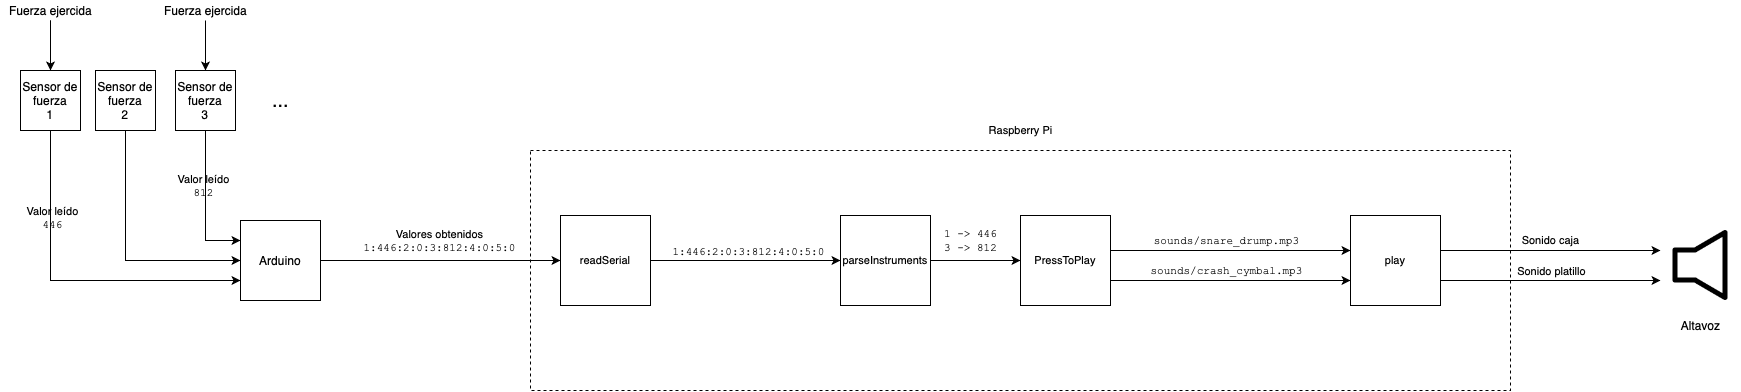
\includegraphics[width=\textwidth]{diagrama_flujo}
            \caption{Diagrama de flujo\label{fig:DiagramaFlujo}}
        \end{figure}

    % section Reproducción de sonido (end)

    \section{Sonido en paralelo} % (fold)
    \label{sec:SonidoEnParalelo}

        Hasta febrero, todas las versiones del programa fueron diseñadas pensando solo en emitir un sonido cada vez,
        pero lo preferible en un proyecto como este es que se emita más de un sonido al mismo tiempo.

        El primer acercamiento fue mediante un sistema de máximos y sonidos combinados. En esta primera solución, se
        escogía el mayor de los seis sonidos y, si había un segundo sonido con un valor mayor que 200 (el mínimo para
        emitir sonido), se enviaba un mensaje a través del log de Arduino seleccionando un sonido combinado. Estos
        sonidos habían sido combinados previamente utilizando los sonidos ya presentes en el proyecto.

        Finalmente, esta solución no funcionó correctamente (no se enviaba la señal del sonido combinado) y se procedió
        a diseñar una nueva. Esta nueva solución es la que se utiliza actualmente en el proyecto. Consiste en mandar
        todas las señales al mismo tiempo. Antes de la implementación de esta solución, el log era así:

        \begin{verbatim}
        0:0
        0:0
        2:364
        0:0
        0:0
        \end{verbatim}

        En este mensaje, se indica que el pad 2 registra una presión de intensidad 364 (sobre 1023). Los \texttt{0:0}
        indican que ningún pad registra presión.

        Tras la implementación de la solución, el log es así:

        \begin{verbatim}
        0:0
        0:0
        1:446:2:0:3:812:4:0:5:0
        0:0
        0:0
        1:0:2:0:3:0:4:902:5:0
        0:0
        \end{verbatim}

        En estos mensajes se envía la siguiente información:
        
        \begin{enumerate}
            \item Los mensajes de \texttt{0:0} indican que ningún pad registra presión.
            \item El primer mensaje indica que se han tocado:
            \begin{itemize}
                \item El pad 1 con intensidad 446
                \item El pad 2 no registra presión
                \item El pad 3 con intensidad 812
                \item El pad 4 no registra presión
                \item El pad 5 no registra presión
            \end{itemize}
            \item El segundo mensaje indica que se han tocado:
            \begin{itemize}
                \item El pad 1 no registra presión
                \item El pad 2 no registra presión
                \item El pad 3 no registra presión
                \item El pad 4 con intensidad 902
                \item El pad 5 no registra presión
            \end{itemize}
        \end{enumerate}

        En cuanto un sensor detecta una presión mayor a 200, se manda el mensaje de todos los sensores al mismo tiempo.
        En caso de que el valor leído sea menor que 200, se manda como 0, pero si es mayor, se manda con los demás. Este
        mensaje es leído y procesado por la Raspberry Pi, que lanzará los procesos necesarios con los sonidos que hagan
        falta según los sensores que hayan sido presionados.

        Con esta segunda propuesta, el programa envía correctamente la señal de todos los sensores y los sonidos son
        emitidos correctamente.

    % section Sonido en paralelo (end)

    \section{Principales problemas} % (fold)
    \label{sec:PrincipalesProblemas}

        \subsection{Número de lecturas en botones} % (fold)
        \label{sub:NumeroDeLecturasEnBotones}

            En el prototipo con botones, al pulsar o dejar pulsado un botón, el programa reproduciría el mismo
            sonido muchas veces. Para solucionar esto se crea una hebra por cada botón, cuando se pulsa, entrará
            en un bucle infinito del que no saldrá hasta que el botón no sea soltado. Al usarse hebras, nos
            permite pulsar más botones al mismo tiempo.

        % subsection Número de lecturas en botones (end)

        \subsection{Hebras vs procesos} % (fold)
        \label{sub:HebrasVSProcesos}

            La primera aproximación a cómo realizar este proyecto fue usando hebras para lanzar los sonidos al mismo
            tiempo, por ser más ligeras, en cuanto a uso de recursos, que los procesos. Sin embargo, debido a la
            implementación de biblioteca utilizada para reproducir sonidos, al lanzar hebras para reproducir varios
            sonidos al mismo tiempo, se producía un error de \textit{segmentation fault}. La solución a este problema
            fue sustituir las hebras por procesos.

        % subsection Hebras vs procesos (end)

        \subsection{Número de lecturas en sensores} % (fold)
        \label{sub:NumeroDeLecturasEnSensores}

            El sensor de presión devuelve muchas lecturas por segundo. Para solucionar esto a la hora de reproducir los
            sonidos hay dos formas de solucionarlo: una es introduciendo un \textit{delay} lo suficientemente grande
            para diferenciar dos toques del sensor, la otra solución, que ha sido la implementada, trata de bloquear el
            sensor cada vez que se entra en uno de los tres intervalos de volumen que se han elegido. Cada vez que entra
            en uno de estos intervalos de deja de leer hasta que no baje la presión lo suficiente. Si la presión sube,
            tampoco enviará señal para que reproduzca sonido.

        % subsection Número de lecturas en sensores (end)

        \subsection{Construcción de paths} % (fold)
        \label{sub:ConstruccionDePaths}

            Al añadir el sensor y el Arduino, el programa que controlaba los sonidos emitidos recibía las mediciones
            del Arduino y, dependiendo de los datos entregados por éste, se emite un sonido a un volumen concreto.
            La construcción de la cadena de texto que contenía el \textit{path} se hacía mediante las funciones de
            copia y concatenación \textit{strcat} y \textit{strdup}. El problema es que al recibir el \textit{path},
            la biblioteca de reproducción de sonidos lanzaba el siguiente error:

            \begin{verbatim}
            malloc(): corrupted top size
            make: *** [Makefile:19: run] Segmentation fault
            \end{verbatim}

            Tras muchas pruebas, como aumentar la cantidad de memoria reservada para el \textit{path} o para el
            buffer que se utiliza en la función de reproducción, o probar a que siempre se enviara el mismo path,
            sin leer del Arduino (reproduciendo el sonido satisfactoriamente), finalmente se decide cambiar la forma en
            la que se genera el path, \textit{hardcodeándolo} en el programa. Esto resulta funcionar y es la solución
            que ha sido implementada en el programa.

        % subsection Construcción de paths (end)

    % section Principales problemas (end)

    \section{Pads} % (fold)
    \label{sec:Pads}

        Los pads son las superficies que son golpeadas para generar los sonidos. Para este proyecto se han fabricado
        usando madera, cola y gomaeva \cite{GomaEva}. El coste total de fabricar un pad es de 1,54\euro{}. Comparado
        con otros productos similares como los de Prologix \cite{practice_pad}, cuyo kit de práctica de 4 pads cuesta
        \$224,99, el precio de la solución propuesta en este proyecto es sensiblemente inferior.

        \subsection{Madera MDF} % (fold)
        \label{sub:MaderaMDF}

            La madera utilizada para fabricar los pads es de tipo MDF. Este tipo de madera se refiere a tableros
            fabricados utilizando fibras de madera y resinas sintéticas para aportar una mayor
            resistencia \cite{mdf_santana}.

            \newpage

            \begin{figure}[ht]
                \centering
                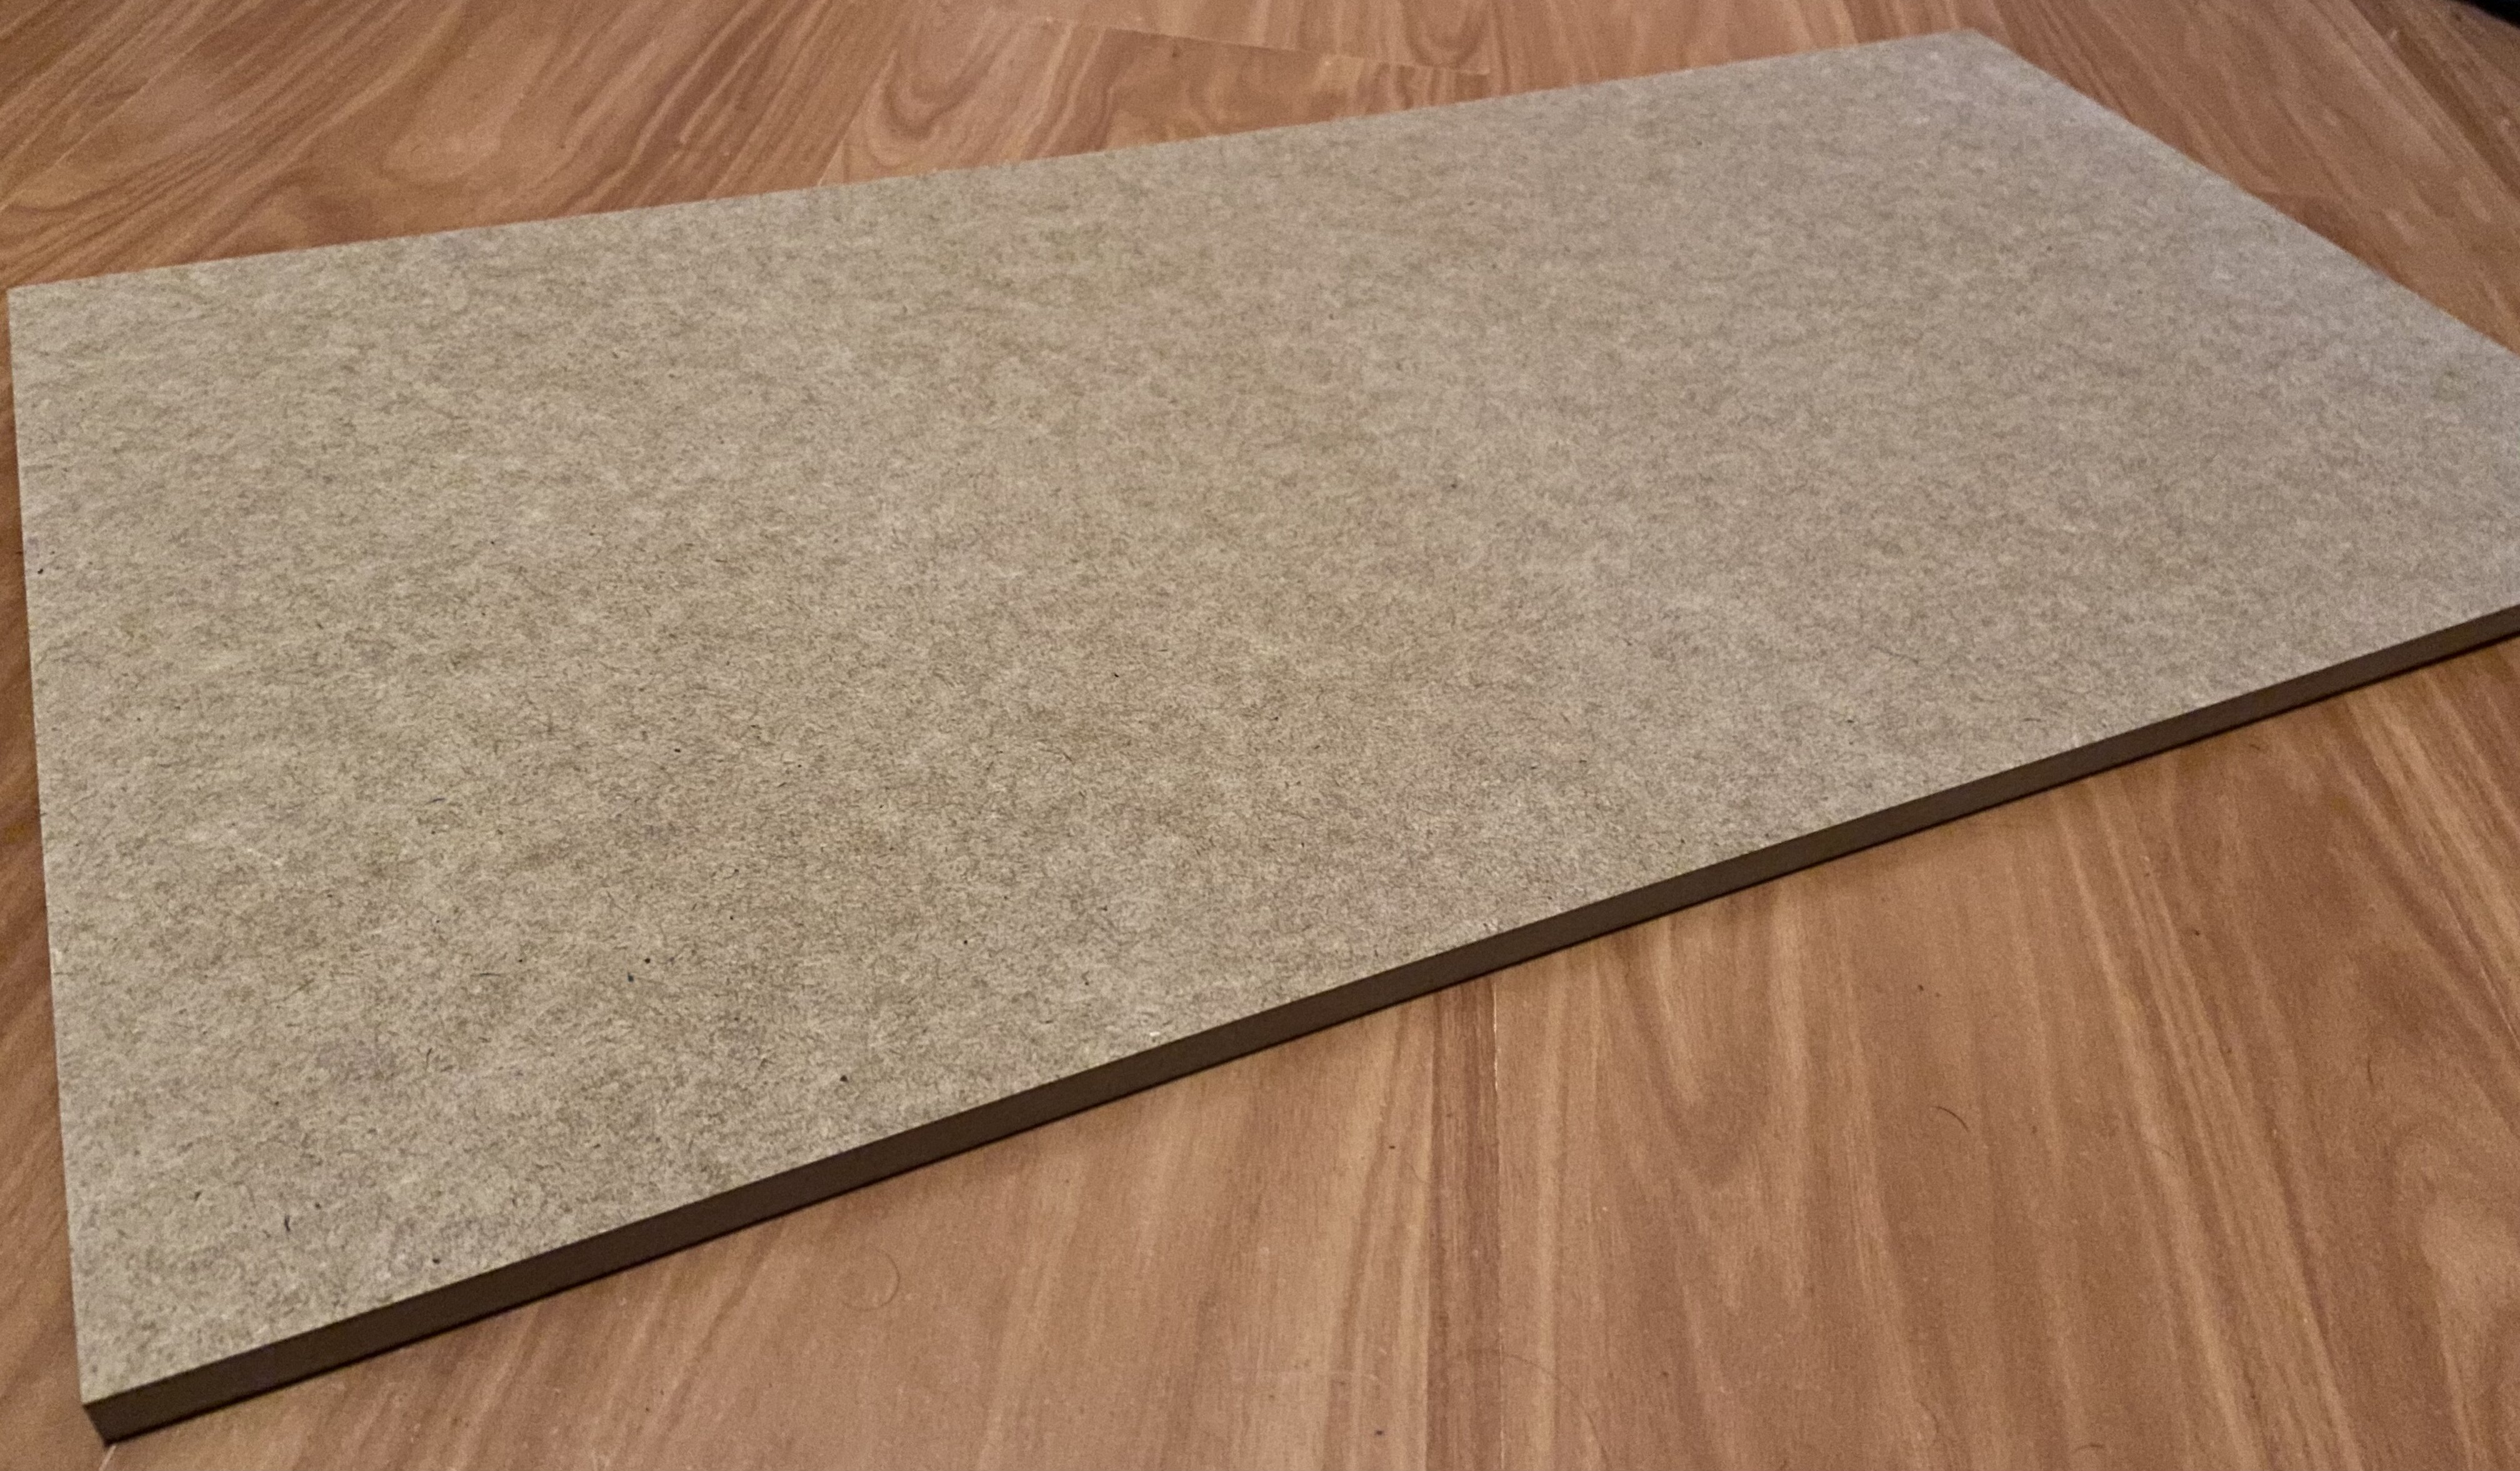
\includegraphics[width=\textwidth]{tablero_mdf}
                \caption{Imagen de tablero MDF\label{fig:TableroMDF}}
            \end{figure}

        % subsection Madera MDF (end)

        \subsection{Construcción} % (fold)
        \label{sub:ConstruccionPads}

            Los pads están hechos a partir de un tablero de madera MDF de 600x300x10 mm. Este tablero se cortó en un
            principio en dos círculos de unos 20 cm de diámetro, con la intención de tener unos sensores de fuerza lo
            suficientemente grandes como para tener sensibilidad de la mayor parte de estos pads. Sin embargo, los
            sensores que finalmente se han usado en el proyecto son más pequeños de lo esperado inicialmente, de
            4x5,5 cm. Debido a esto, se tuvieron que recortar nuevos pads más pequeños, para que los sensores cubrieran
            la mayor area del pad posible. Estos nuevos pads contaban con unos 12 cm de diámetro. El resultado después
            de recortarlos es el indicado en la figura \ref{fig:PadsRecortados}.

            \begin{figure}[ht]
                \centering
                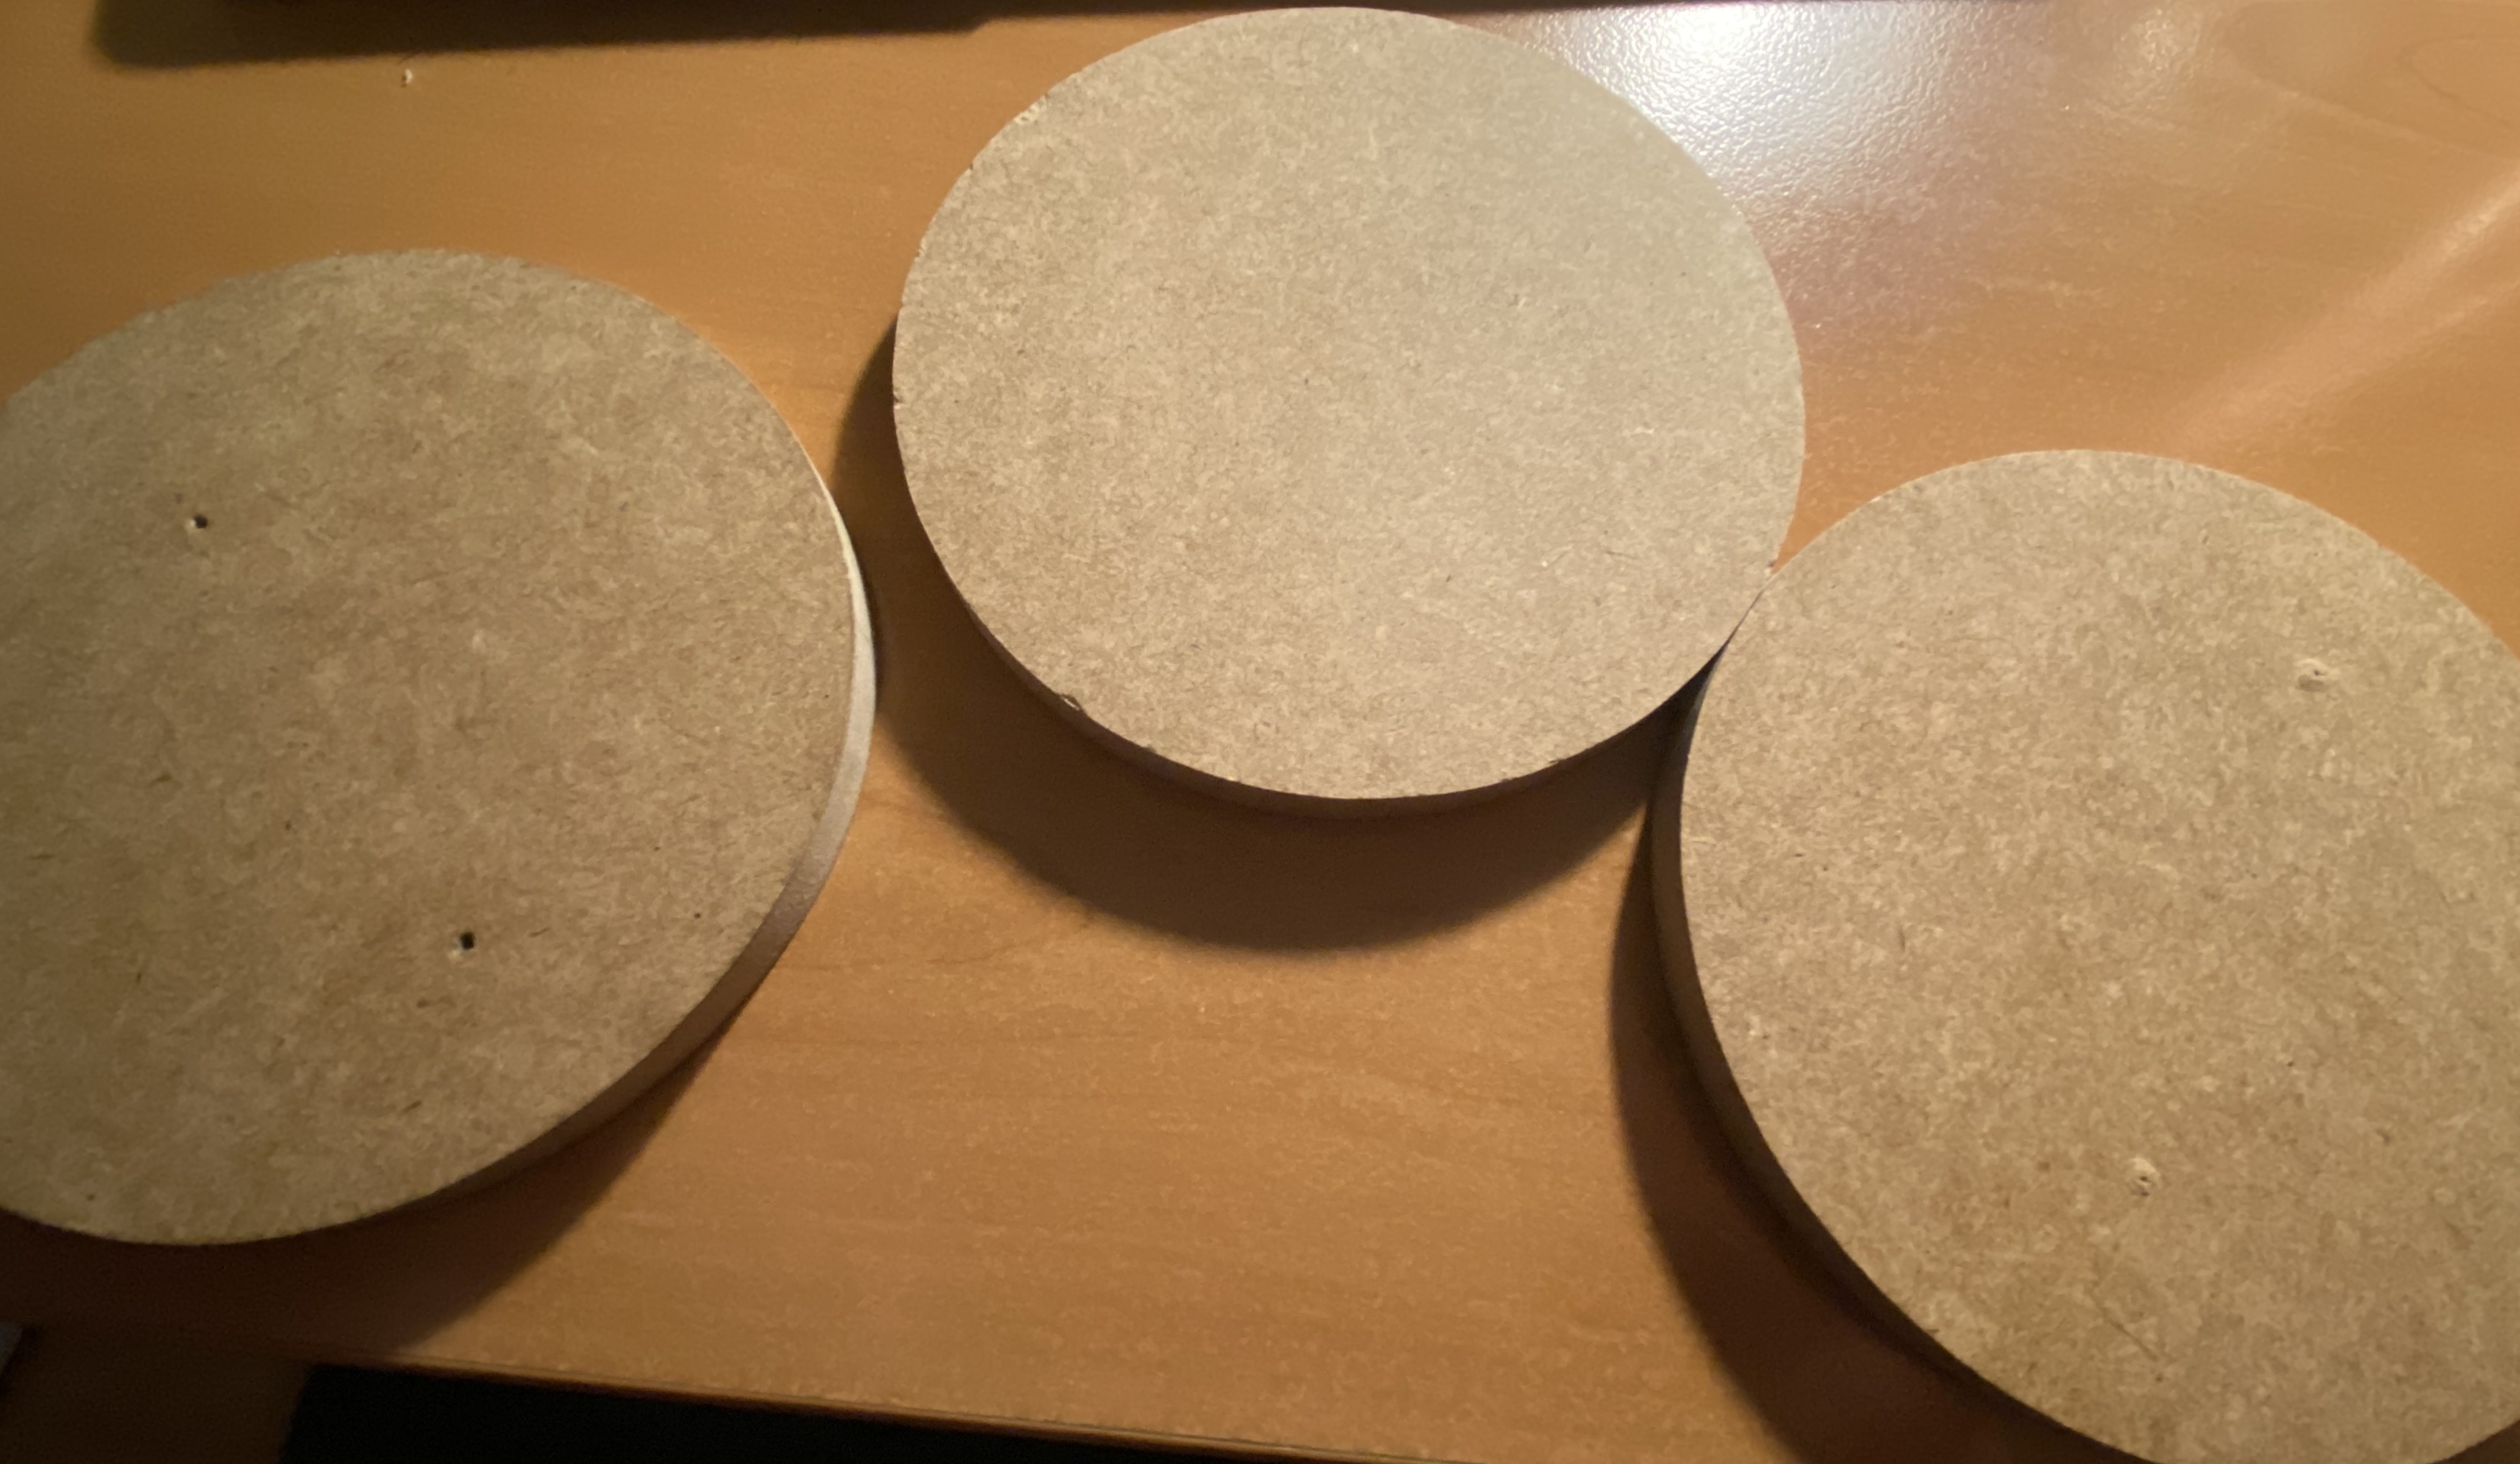
\includegraphics[width=\textwidth]{pads_recortados}
                \caption{Imagen de los pads una vez recortados\label{fig:PadsRecortados}}
            \end{figure}

            \newpage

            Tras ser recortados, el siguiente paso es añadir agujeros en el pad para que pasen los cables del sensor.
            Estos agujeros hacen que, cuando se golpea el pad con la baqueta, se reduzca la posibilidad de dañar los
            cables debido a los golpes. El resultado es el de la figura \ref{fig:PadsAgujeros}

            \newpage

            \begin{figure}[ht]
                \centering
                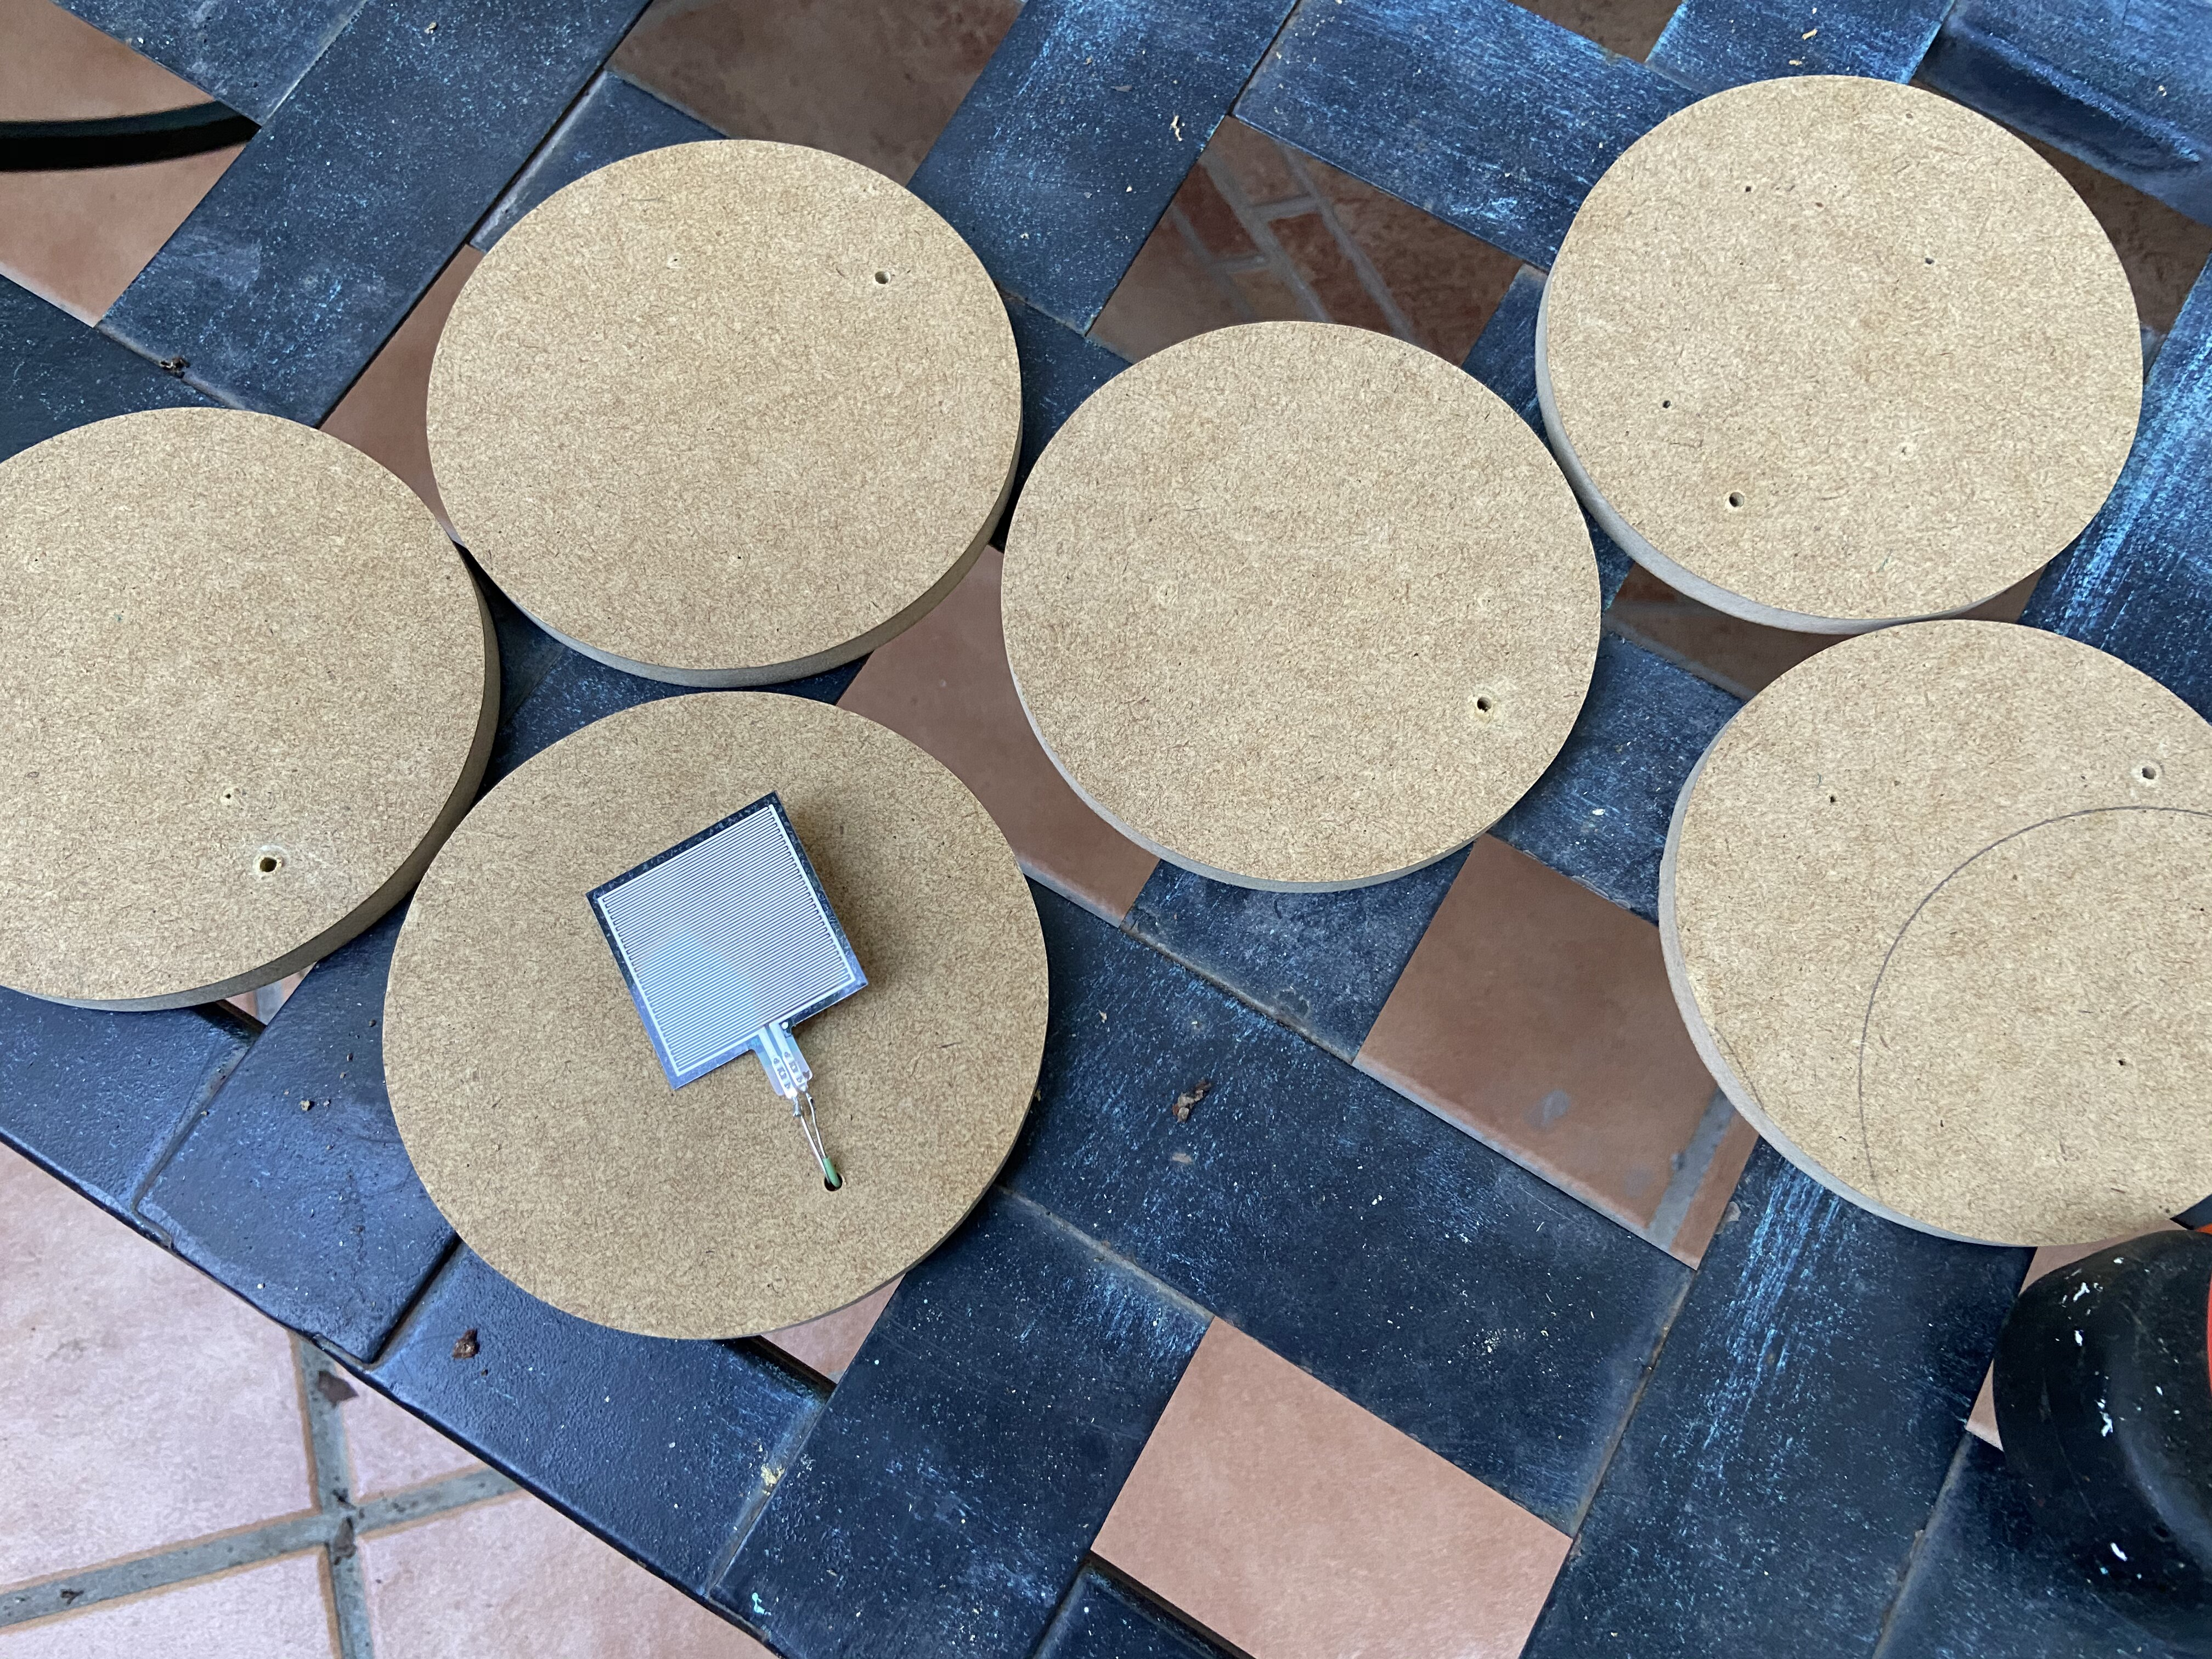
\includegraphics[width=\textwidth]{pads_con_agujeros}
                \caption{Imagen de los pads y un sensor tras añadir los agujeros\label{fig:PadsAgujeros}}
            \end{figure}

            Una vez hecho eso, se añade la gomaeva para proteger los sensores y dar una mayor sensación de realismo al
            ser golpeado con la baqueta.

            --- Imagen aquí ---
            %%%%%%%%%%%%%%%%%%%%%%%%%%%%%%%%%%
            % Imagen de los pad con la gomaeva
            %%%%%%%%%%%%%%%%%%%%%%%%%%%%%%%%%%

        % subsection Construcción (end)

    % section Pads (end)

    \section{Tiempo} % (fold)
    \label{sec:Tiempo}

        Para medir el tiempo que ha llevado realizar este trabajo, se ha utilizado la aplicación
        Clockify \cite{clockify}.\newline

        En total se han utilizado 113 horas y 54 minutos.%%%%%%%%%%%%%%%%%%%%%%%%%%%%%%%%%%%%%%%%%%%%%%%%%%%%%%
        %%%%%%%%%%%%%%%%%%%%%%%%%%%%%%%%%%%%%%%%%%%%%%%%%%%%%%%%%%%%%%%%%%%%%%%%%%%%%%%%%%%%%%%%%%%%%%%%%%%%%%
        %%%%%%%%%%%%%%%%%%%%%%%%%%%%%%%%%%%%%%%%%%%%%%%%%%%%%%%%%%%%%%%%%%%%%%%%%%%%%%%%%%%%%%%%%%%%%%%%%%%%%%

    % section Tiempo (end)

    \section{Coste y presupuesto} % (fold)
    \label{sec:CosteYPresupuesto}

        tabla con el coste de desarrollo (incluye tu mano de obra... etc.)

        \subsection{Materiales} % (fold)
        \label{sub:Materiales}

            \begin{itemize}
                \item Dos hojas de goma eva: 1,20\euro{}
                \item Tres tablas madera MDF 600x300x10 mm: 7,47\euro{}
                \item Cables protoboard: 2,60\euro{}
                \item Sensor de fuerza Exing c18.3: 5,91\euro{}
                \item Tres sensores de fuerza Exing RP de S40: 50,95\euro{}
                \item Raspberry Pi 3B: 39,95\euro{}
                \item Tarjeta micro SD 8 GB: 5\euro{}
                \item Caja Aukru + cable alimentación: 11,99\euro{}
                \item Arduino Nano: 15,43\euro{} (incluye gastos de envío)
            \end{itemize}

            El coste de los materiales se queda, finalmente, en 140,50\euro{}.

        % subsection Materiales (end)

    % section Coste y presupuesto (end)

% chapter Implementación (end)

\newpage
